\documentclass[10pt,twocolumn,letterpaper]{article}

\usepackage[monochrome]{color}

\usepackage{hhline}
\usepackage{wacv}
\usepackage{subcaption}
\usepackage{graphics} % for pdf, bitmapped graphics files
\usepackage{epsfig} % for postscript graphics files
\usepackage{mathptmx} % assumes new font selection scheme installed
\usepackage{times} % assumes new font selection scheme installed
\usepackage{amsmath} % assumes amsmath package installed
\usepackage{amssymb}  % assumes amsmath package installed
\usepackage{booktabs}
\usepackage{multirow}
\usepackage{hyperref}
\usepackage{cleveref}
%\usepackage{flushend}
\usepackage{afterpage}
\usepackage{dblfloatfix}    % To enable figures at the bottom of page

% Include other packages here, before hyperref.

% If you comment hyperref and then uncomment it, you should delete
% egpaper.aux before re-running latex.  (Or just hit 'q' on the first latex
% run, let it finish, and you should be clear).
%\usepackage[pagebackref=true,breaklinks=true,letterpaper=true,colorlinks,bookmarks=false]{hyperref}


\wacvfinalcopy % *** Uncomment this line for the final submission

\def\wacvPaperID{****} % *** Enter the wacv Paper ID here
\def\httilde{\mbox{\tt\raisebox{-.5ex}{\symbol{126}}}}

% Pages are numbered in submission mode, and unnumbered in camera-ready
\ifwacvfinal\pagestyle{empty}\fi
\setcounter{page}{1}
\begin{document}

%%%%%%%%% TITLE
\title{MultiNet: Multi-Modal Multi-Task Learning for Autonomous Driving}

% Authors at the same institution
%\author{First Author \hspace{2cm} Second Author \\
%Institution1\\
%{\tt\small firstauthor@i1.org}
%}
% Authors at different institutions
\author{Sauhaarda Chowdhuri \\
Berkeley DeepDrive Center\\
{\tt\small sauhaarda@berkeley.edu}
\and
Tushar Pankaj \\
Berkeley DeepDrive Center\\
{\tt\small tpankaj@berkeley.edu}
\and
Karl Zipser \\
Berkeley DeepDrive Center\\
{\tt\small karlzipser@berkeley.edu}
}

\maketitle
\ifwacvfinal\thispagestyle{empty}\fi


%%%%%%%%% ABSTRACT
\begin{abstract}
Several deep learning approaches have been applied to the autonomous driving task, many employing end-to-end deep neural networks. Autonomous driving is complex, utilizing multiple behavioral modalities ranging from lane changing to turning and stopping. However, most existing approaches do not factor in the different behavioral modalities of the driving task into the training strategy. This paper describes a technique for using Multi-Modal Multi-Task Learning, which we denote as MultiNet which considers multiple behavioral modalities as distinct modes of operation for an end-to-end autonomous deep neural network utilizing the insertion of modal information as secondary input data. Using labeled data from hours of driving our fleet of 1/10th scale model cars, we trained different neural networks to imitate the steering angle and driving speed of human control of a car. We show that in each case, MultiNet models outperform networks trained on individual tasks, while using a fraction of the number of parameters.
\end{abstract}


%The salamander is capable of rapidly switching between two locomotion modes: swimming and walking. The muscle movements required for locomotion are executed by the spinal chord and the modal information for which action to execute is delivered by the salamander brain. We attempt to imitate this modal switching behavior of the salamander spinal chord in our own self driving network by feeding in behavioral information to the network. In this case we used two easily distinguishable behavioral modes, follow and direct in contrast to swimming and walking for the salamander. The follow behavioral mode consists of data with our car following another car in front of it, when this car slows down our car should slow down and should follow close behind it. The direct behavioral mode consists of data with the network driving itself on paths at a relatively constant speed.
%For our base network, we used SqueezeNet \cite{iandola2016squeezenet}, since it is a compact network with large receptive fields, and it has shown to be good at regression tasks. The network is slightly modified to allow for 12 channels of input (RGB Color, Left/Right, and current/previous time step). For our MTL network we modified the structure further to support insertion of modal information after the network has done initial processing of visual data.


\section{INTRODUCTION}
\label{sec:intro}


%Learning complex autonomous behaviors like driving, is an ongoing research topic in computer vision and machine learning. Learning based approaches are most effective for dealing with complex or rare scenarios.

Most current research on driving with DNNs has focused on a single driving modality, e.g.\ lane following or obstacle avoidance \cite{bojarski2016end,muller2006off,chen2015deepdriving,DBLP:journals/corr/HuvalWTKSPARMCM15}. We consider these approaches as \textit{Single Task Learning} (STL), as they focus on training to perform an individual task.

%------>In contrast, several methods for other learning problems have learnt multiple tasks simultaneously, in an approach known as Multi Task Learning (M
Multi-task learning (MTL) research has shown that training on side tasks related to the main operation of a deep neural network can enhance its learning capabilities \cite{caruana1998multitask, zhang2012convex}. These side tasks, such as finding the position of sidewalks in the image in addition to driving with lane following, may allow networks to break down image processing into stages and develop specific filters for individual steps in a processing pipeline. In MTL, these side tasks are not used when evaluating networks in inference mode and instead improve performance on the primary task; e.g.\ steering angle prediction.

\begin{figure}[t]
\centering
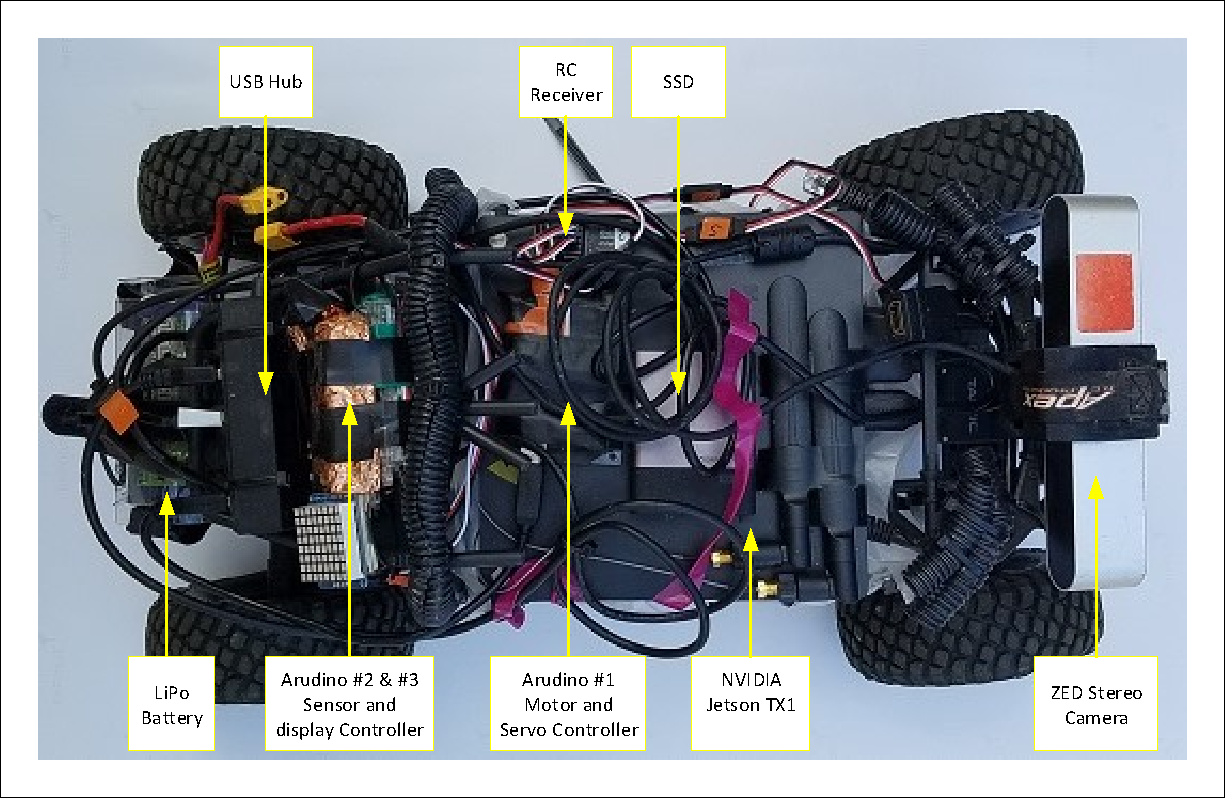
\includegraphics[width=\linewidth,,trim=20 20 20 20,clip]{paper/content/images/car}
\caption{Car Diagram}
\label{fig:cars}
\end{figure}

\afterpage{
\begin{figure*}[!th]
\centering
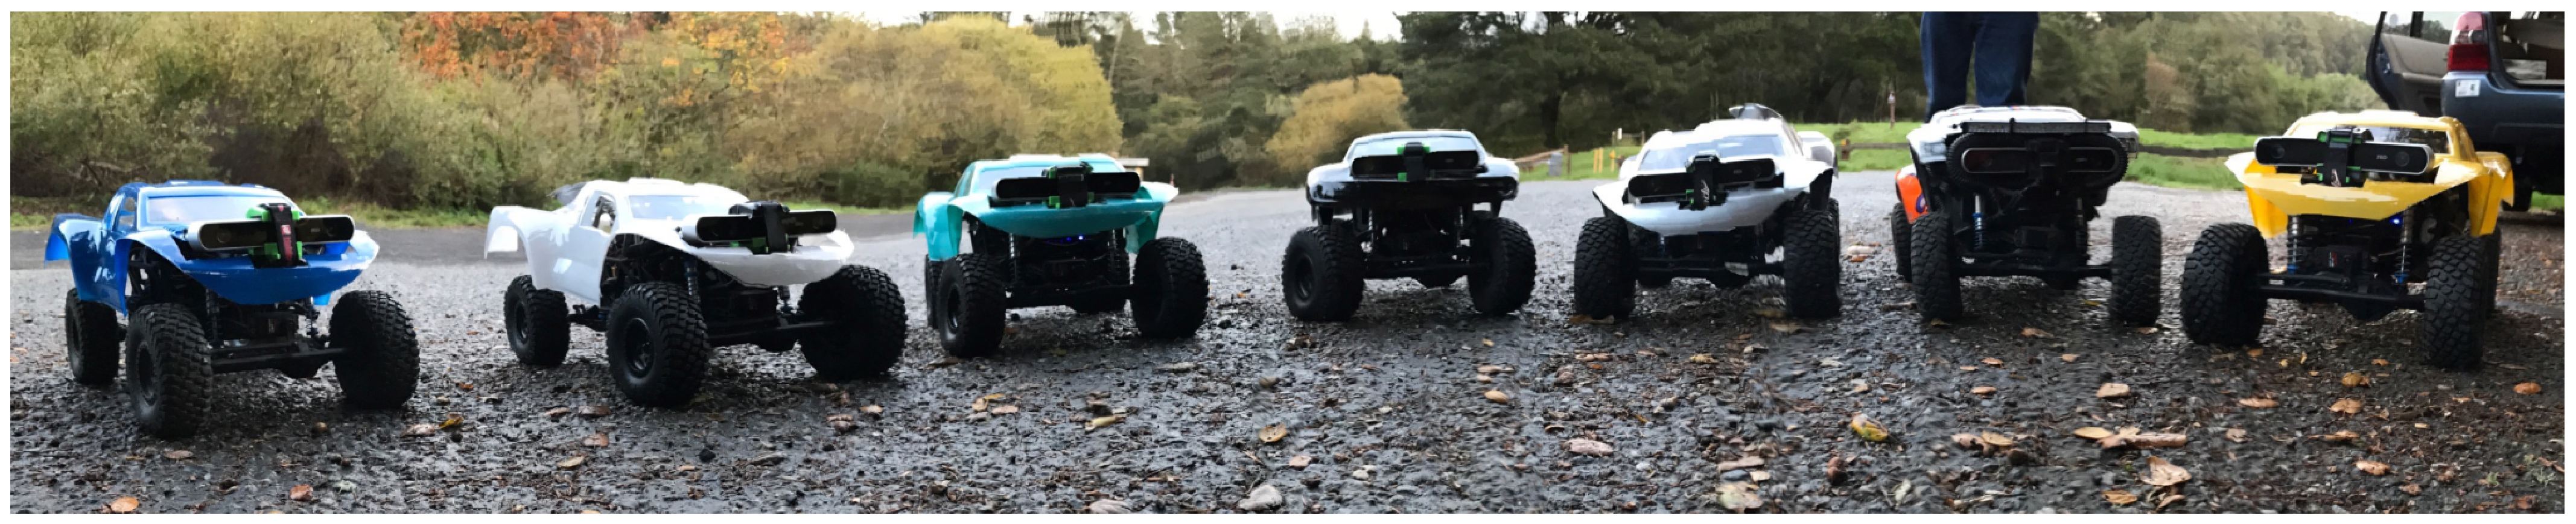
\includegraphics[width=0.9\textwidth]{paper/content/images/fleet}
\caption{Fleet of Model Cars}
\label{fig:fleet}
\end{figure*}
\begin{figure*}[!th]
    \centering
     \begin{subfigure}{0.3\textwidth}
       \centering
       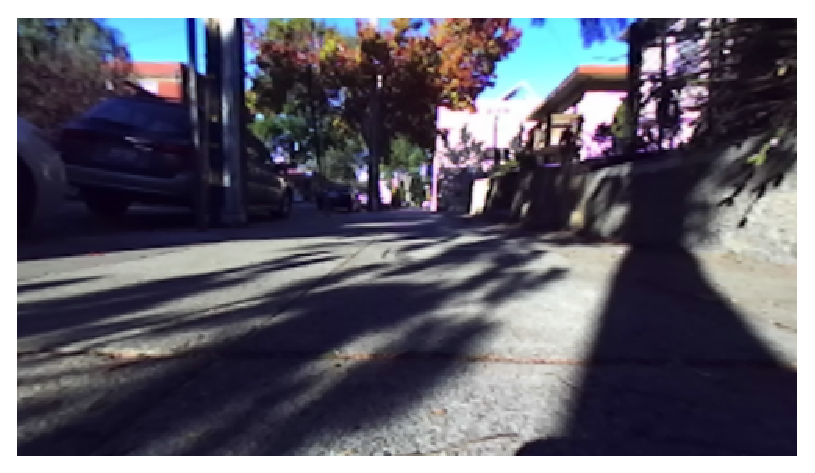
\includegraphics[width=\linewidth]{paper/content/images/daytime}
       \caption{Day Time}
     \end{subfigure}
     \begin{subfigure}{0.3\textwidth}
       \centering
       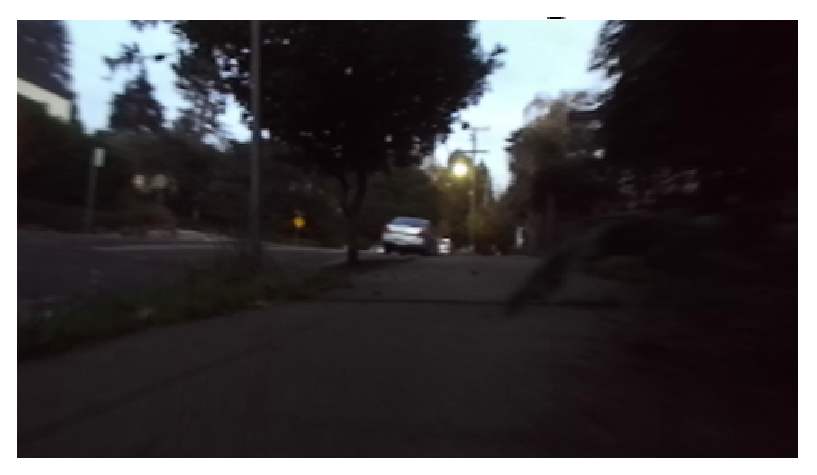
\includegraphics[width=\linewidth]{paper/content/images/evening}
       \caption{Evening}
     \end{subfigure}
     \begin{subfigure}{0.3\textwidth}
       \centering
       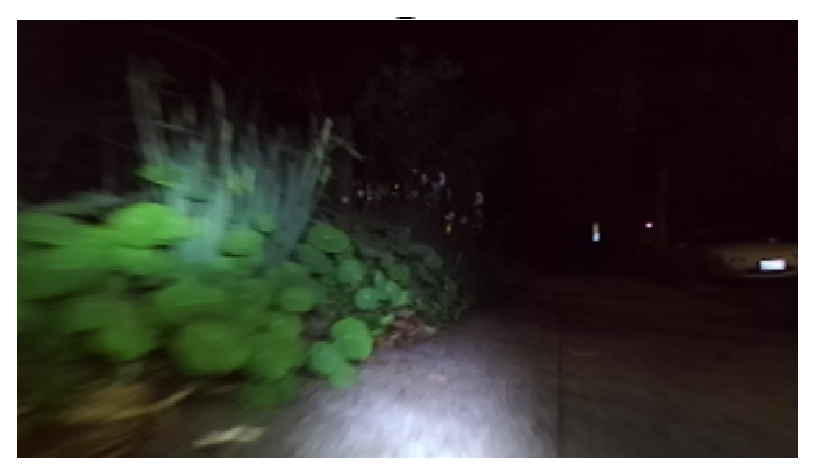
\includegraphics[width=\linewidth]{paper/content/images/night}
       \caption{Night Time}
     \end{subfigure}
        \begin{subfigure}{0.3\textwidth}
       \centering
       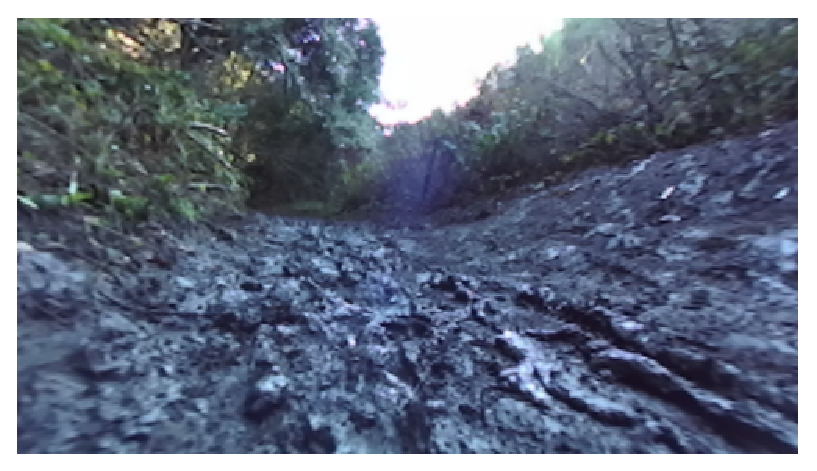
\includegraphics[width=\linewidth]{paper/content/images/muddy}
       \caption{Muddy Area}
    \end{subfigure}
    \begin{subfigure}{0.3\textwidth}
       \centering
       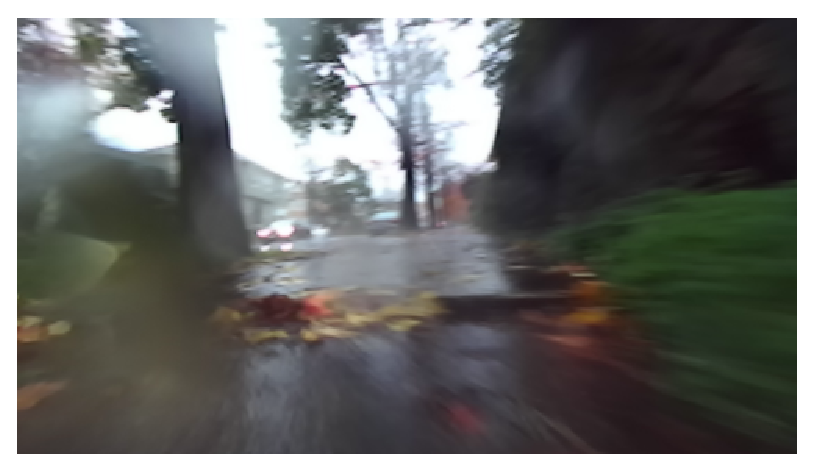
\includegraphics[width=\linewidth]{paper/content/images/rainy}
       \caption{Rainy Area}
    \end{subfigure}
    \begin{subfigure}{0.3\textwidth}
       \centering
       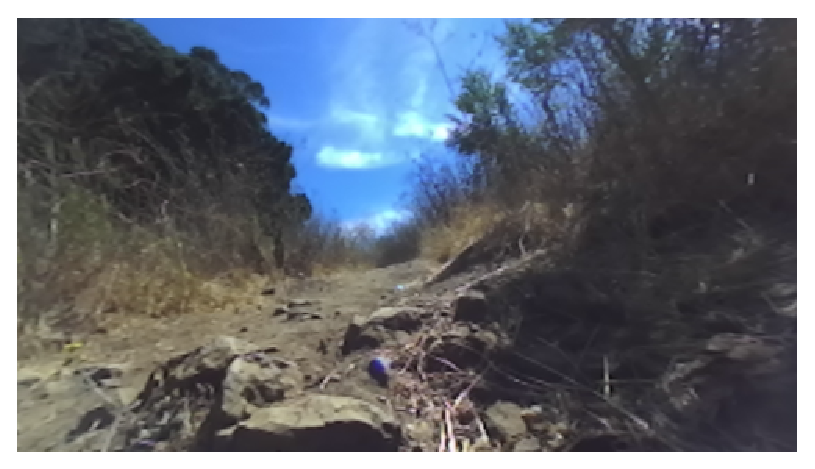
\includegraphics[width=\linewidth]{paper/content/images/bumpy}
       \caption{Bumpy Area}
    \end{subfigure}
    \caption{Diverse Conditions in Dataset}
    \label{fig:diverse}
\end{figure*}

\begin{figure*}[!th]
    \centering
    \begin{subfigure}{0.3\textwidth}
       \centering
       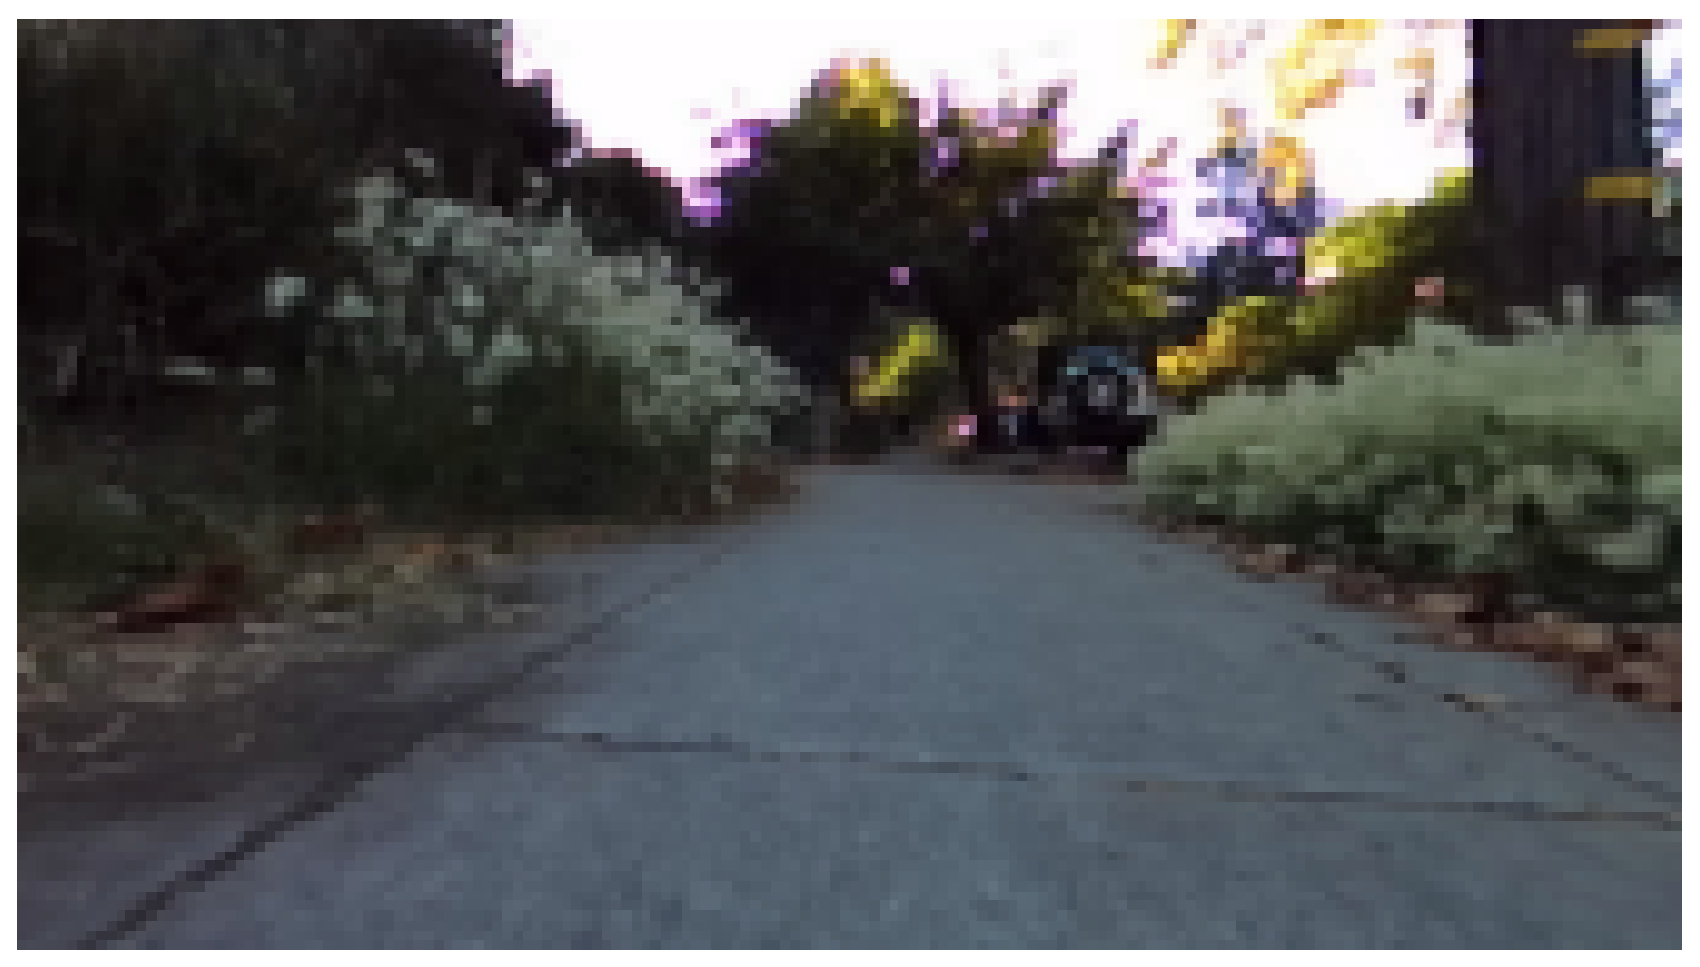
\includegraphics[width=\linewidth]{paper/content/images/directexample}
       \caption{Direct Mode}
       \label{fig1:direct}
    \end{subfigure}
    \begin{subfigure}{0.3\textwidth}
       \centering
       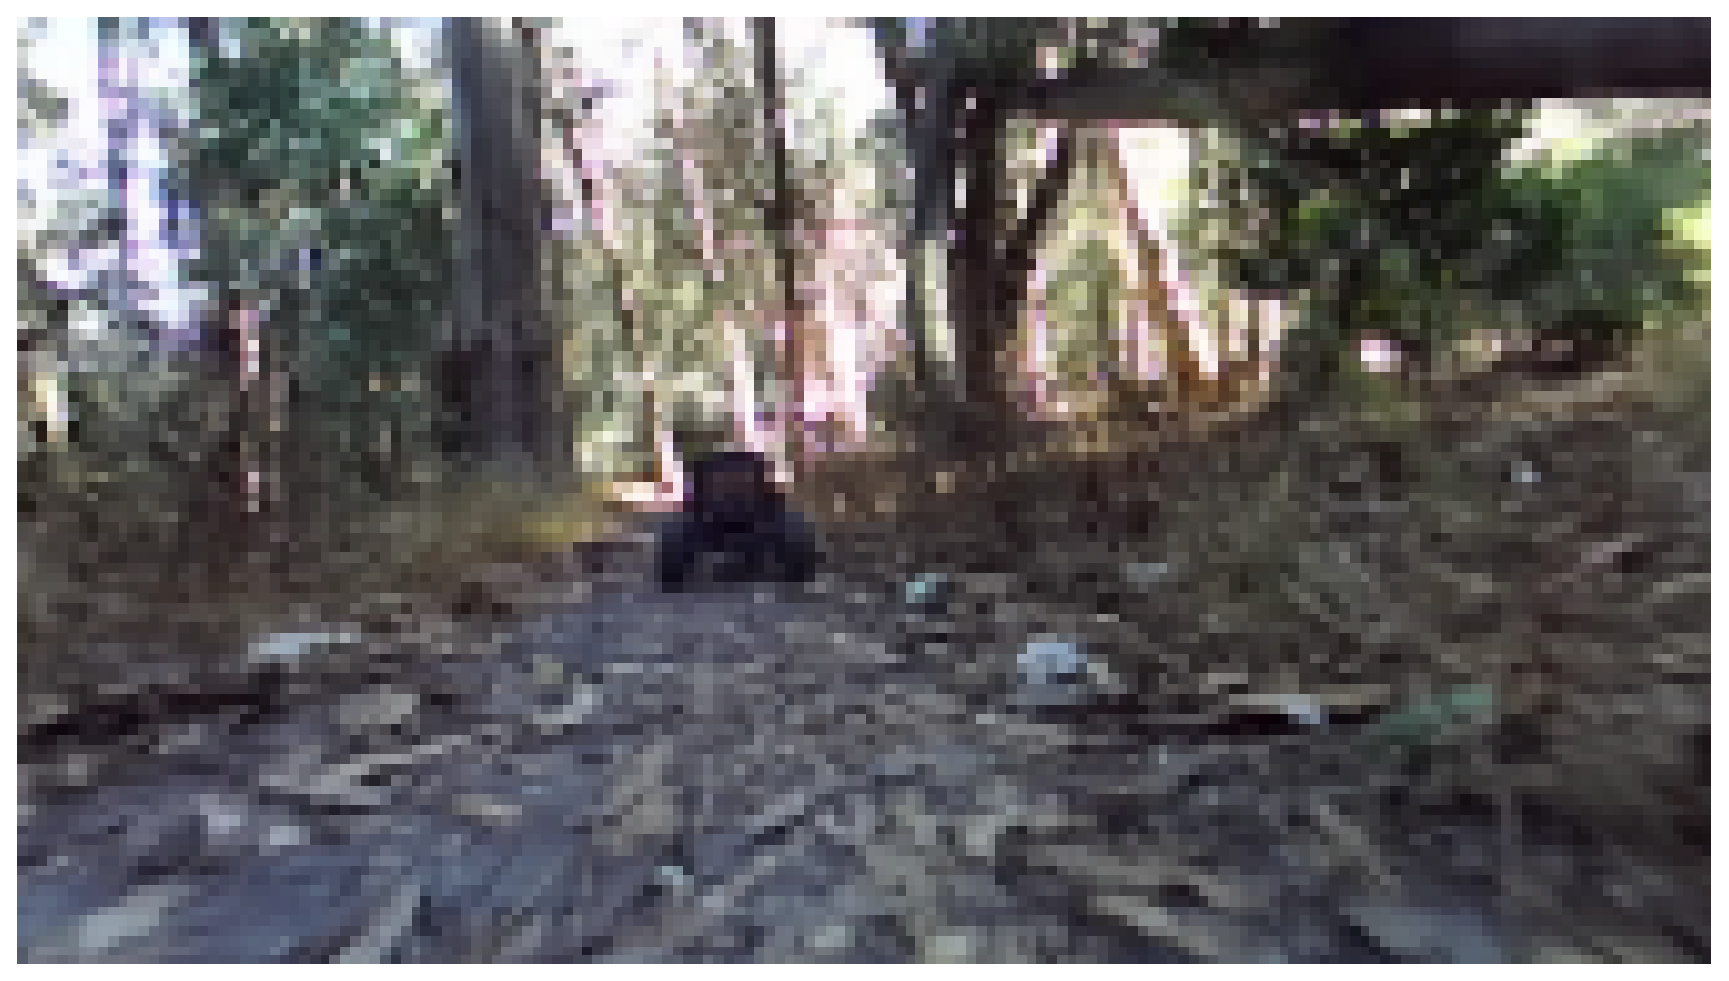
\includegraphics[width=\linewidth]{paper/content/images/followexample}
       \caption{Follow Mode}
       \label{fig1:follow}
    \end{subfigure}
    \begin{subfigure}{0.3\textwidth}
       \centering
       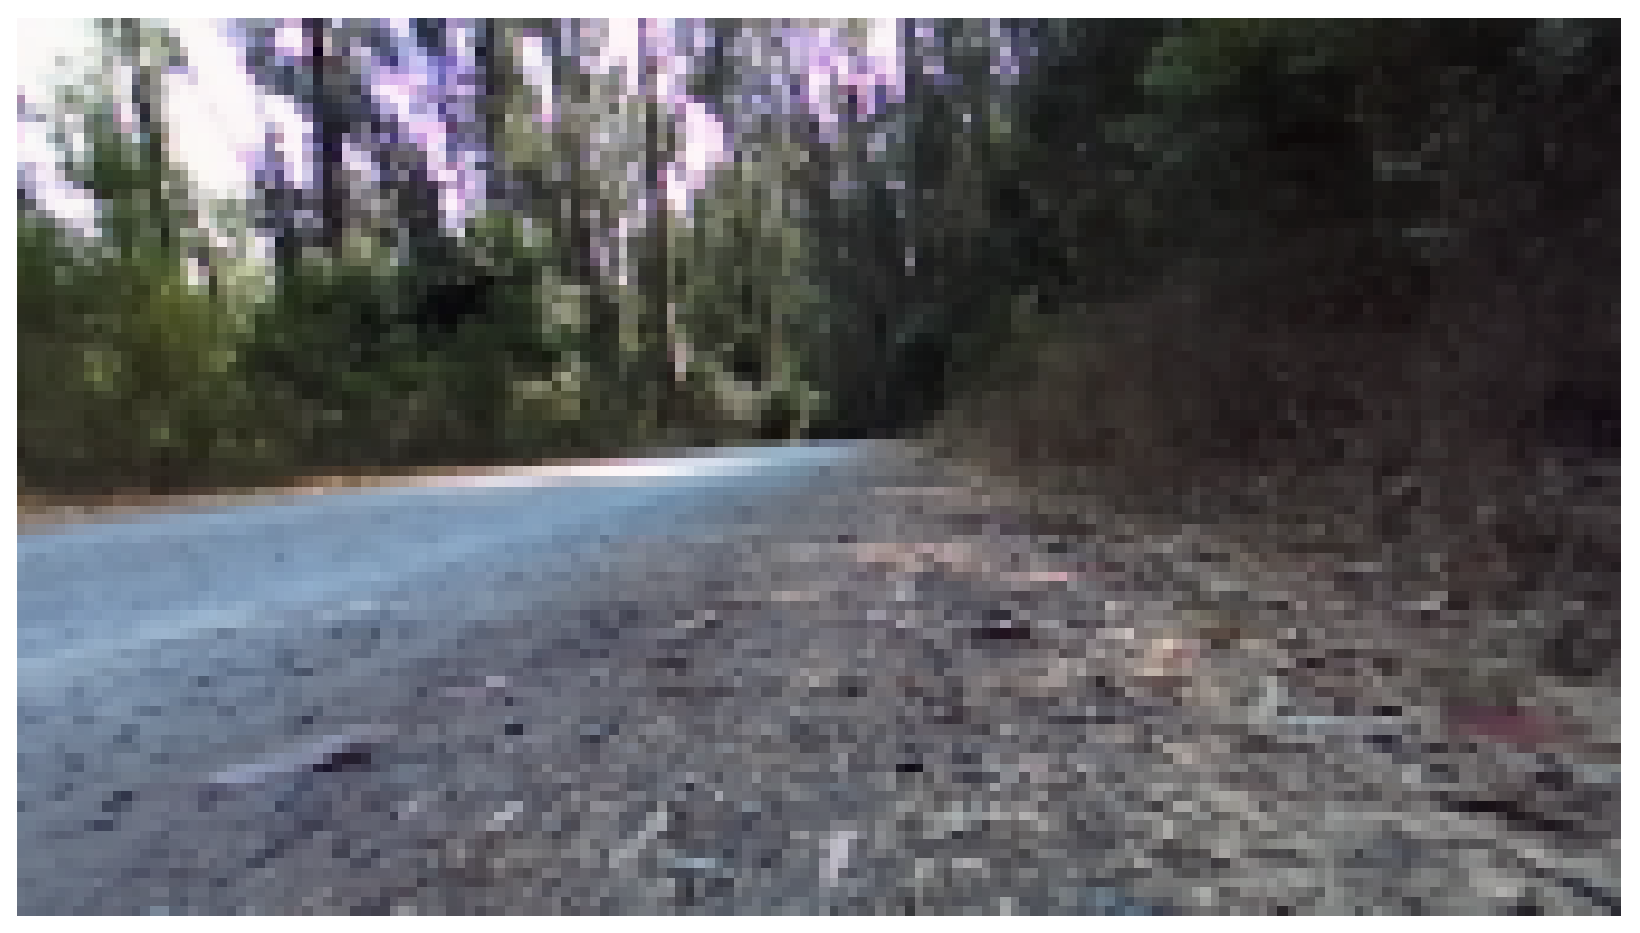
\includegraphics[width=\linewidth]{paper/content/images/furtiveexample}
       \caption{Furtive Mode}
       \label{fig1:furtive}
    \end{subfigure}
    \caption{Behavioral Mode Sample Data from Car's Point of View}
    \label{fig1:behavioralmodes}
\end{figure*}
}

Additional research is being conducted on multi-modal learning, a method in which networks are trained on several distinct modes of operation, all of which are used during inference.
For example, a network which has the single task of transcribing audio to text may be given a side task of sentiment analysis to improve performance in the transcribing task \cite{6639012}. This is a multi-task learning network as the side-task of sentiment analysis is not needed during inference and is merely used to improve performance on a different task. If instead the network is given the task of transcribing text in two modes: one for audio, and the other for video recordings \cite{ngiam2011multimodal}. This is an example of multi-modal learning as there are multiple modes of running the network either of which can be used during evaluation.

Work on multi-modal learning has predominantly been focused in fields other than robotics or locomotion; e.g.\ speech recognition with audio and video \cite{ngiam2011multimodal, 6639012}. Within these works, it is common for DNNs to be given input that could correspond to any or multiple modes of operation. 

In the context of performing multiple tasks multi-modal networks have significantly fewer parameters when compared to systems with multiple networks, as multiple related tasks can be completed by a single network rather than multiple networks. Smaller network sizes are desirable as they allow for fast over the air model updates in self driving cars, and deployment on Field Programmable Gate Arrays (FPGA) \cite{DBLP:journals/corr/IandolaMAHDK16}.
% The MTL side tasks consist of additional motor and steering values inferred by the network, which are not used for actuation on the vehicles at the time of evaluation.
In this paper, we propose a new method for combining multi-modal learning with MTL for autonomous driving.
In this method, the MTL side tasks consist of additional motor and steering values inferred by the network, which are not used for actuation on the vehicles at time of evaluation. These side-tasks are akin to sentiment analysis in the prior example.
Additionally, we introduce multiple distinct driving behaviors, or \textit{behavioral modes}, in which the model car can operate.
These behaviors constitute the modes of evaluation for multi-modal learning, akin to audio and video in the previous example.
The behavioral modes are given to the network as a privileged secondary input, allowing for separate driving behaviors to form within a single network.

% In this approach, side tasks consist of separate driving behaviors which are all used during inference. Additionally, the current mode of operation is given to the network as a secondary input, allowing for separate driving behaviors to form within a single network.
We denote our multi-modal MTL networks as \textit{MultiNets} in contrast to the MTL networks trained in a single behavioral mode. We show that in addition to having a size advantage over a simple MTL approach, MultiNets exceed the performance of multiple MTL networks on the same tasks in evaluation on a validation dataset as well as in on-the-road experiments.

The concurrent work of \cite{intel_paper} investigates a multi-modal approach with multiple sub-networks for each mode and provides a mathematical justification for the insertion of privileged modal data. Our approach differs in that a single general and scalable network is used to infer an arbitrary number of behavioral modalities using a novel logical modal switch in the processing stream of the network.

This paper is organized as follows.
Section \ref{sec:dataset} covers the methods of collection of our dataset, as well as detailing the robotic cars used in the work.
Section \ref{sec:approach} describes the specific innovations of MultiNets, as well as introducing our own deep convolutional neural network, \textit{Z2Color}, used for training and running experiments.
Section \ref{sec:experiments} covers the experiments conducted through evaluation of network validation loss for multiple and individual behavioral modes, as well as evaluation in on-the-road tests.
Finally, Section \ref{sec:conclusion} summarizes the major contributions of this paper and suggests areas for future work.
% In the self driving case, researchers have also shown how DNNs can be trained to predict and distinguish between separate driving modalities such as turning or stopping \cite{xu2016end}.



\section{DATASET}
\label{sec:dataset}

\subsection{Fleet of Cars}
The dataset was collected using a fleet of 1/10th scale RC model cars (\Cref{fig:fleet}) similar to that of \cite{intel_paper, williams2017information, giusti2016machine, muller2006off, muller2013real, krasheninnikov2017autonomous} for recording data in unstructured off-road environments as well as sidewalks. \Cref{fig:cars} shows the main sensor and control components of the car. The small size of the model car provides the flexibility to experiment in diverse driving terrains and lighting conditions. Our dataset contains hundreds of hours of data from environments including city sidewalks, parks, forests and snowy environments. Data were collected in different weather conditions and at different times of the day (\Cref{fig:diverse}). Additionally, the small size of the cars allow for experiments with atypical driving behaviors and the collection of data involving the vehicle making and recovering from mistakes.

There are four computing nodes in the car -- one NVIDIA Jetson TX1 \footnote{ TX1 Developer Kit at \url{https://developer.nvidia.com/embedded/buy/jetson-tx1-devkit}} and three Arduino Uno\footnote{Arduino Unos available at \url{https://www.arduino.cc/}} micro-controllers.

The nodes communicate with one another using Robot Operating System (ROS) Kinetic \cite{quigley2009ros}. Arduino \#1 performs pulse width modulation for the steering servo motor and power control of the DC drive motor. It also connects to an RC receiver, through which user steering and drive power commands from the RC transmitter are received. Arduino \#1 provides the RC controller data to the TX1 and receives servo position and motor power information in return. The main sensor for the car is the ZED RGB stereo camera, developed by StereoLabs\footnote{ ZED Stereo Camera from \url{https://www.stereolabs.com/zed/specs/}}, connected to the TX1. There are optional auxiliary sensors, such as the gyroscope and accelerometer, which are controlled by Arduino \#2, although no auxiliary sensors were used for the experiments described in this paper. Arduino \#3 is dedicated to real-time debug message display using an 8x8 LED panel. 

During the data collection process, the car is controlled using an RC Transmitter. Every 33 ms, the left and right RGB images from the stereo camera, along with steering position and motor power level, are saved to on-board SSD storage. The datasets are labelled according to the behavioral mode and operation mode used.

\subsection{Behavioral Modes}

The dataset also contains annotated modes of behavior for the model car to constitute the behavioral modes used during inference for the MultiNets. We use three distinct behavioral driving modes:

\begin{enumerate}
    \item \textbf{Direct Mode} consists of data with the car driving with few obstructions or obstacles, usually on a winding sidewalk or forest path (\Cref{fig1:direct}).
    \item \textbf{Follow Mode} consists of data with the car following a lead car in front of it. In this mode, speed modulation occurs as maintaining an uniform distance from the lead car is attempted during driving (\Cref{fig1:follow}).
    \item \textbf{Furtive Mode} consists of data where the car attempts to drive slowly in close proximity to perceived boundaries e.g.\ shrubbery or bushes on either side of a path. If no such boundaries are identified, the car speeds up along the path until one is found (\Cref{fig1:furtive}).
\end{enumerate}

%\begin{figure}[t]
%   \centering
%   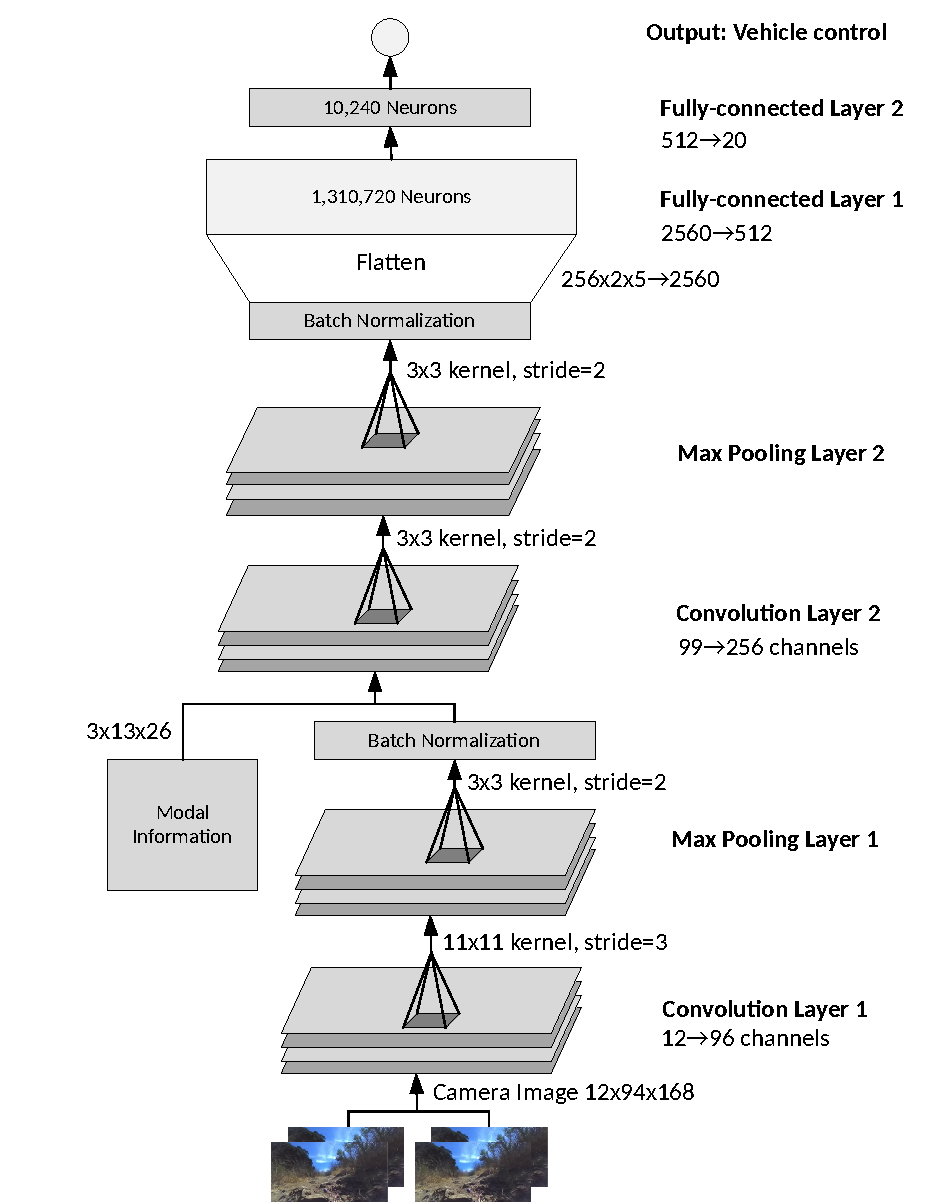
\includegraphics[width=\columnwidth]{paper/content/images/z2color}
%   \caption{Z2Color Network Architecture with Privileged Modal Insertion}
%   \label{fig:squeeze}
%\end{figure}
%

\subsection{Operation Modes}
During data collection runs, the car operates in one of three operational modes: \textit{autonomous}, \textit{expert}, and \textit{correctional}. The autonomous mode is used for evaluating trained networks by allowing a trained network to infer the speed and steering of the model car from the input camera data. During the autonomous mode, the RC receiver remains active, allowing the user to manually override the network's predicted steering values when needed. If a human expert monitoring the car adjusts the speed or steering on the RC transmitter, the car will automatically move into correctional mode allowing for human correction and recovery to avoid the car flipping over or hitting an obstacle. Finally, in the expert mode the expert has full control of the vehicle and records data for future imitation learning.

\subsection{Dataset Aggregation}
Our system utilizes imitation learning. Imitation learning has a basic problem, known as the data mismatch problem, which occurs when a trained network encounters new situations which aren't represented in the dataset of expert driving. In this situation, error compounds quadratically over time to bring the network farther away from expert trajectory \cite{ross2010efficient}.

To solve this problem we implemented a novel approach to the DAgger algorithm \cite{ross2011reduction} which traditionally requires manual labeling of expert trajectories after data are collected from the running network. The small size of the car allowed us to safely record data of the RC vehicle making and recovering from mistakes. New data are then merged with the active dataset for future training in the next iteration. Due to the live corrections, we are able to streamline the data collection process by solving the data mismatch problem while eliminating the need for expert labeling after the data are collected. Our dataset consisted of 19.24\% correctional data and 80.76\% expert data at the time of training and evaluation of the models presented in this paper.

\subsection{Data Moments}

The ROS system gathers time stamps for recorded motor, steer, and camera data. After this data are collected it is processed, interpolated, and synchronized into packets we call \textit{data moments}. We define a data moment as a set of four RGB input images and an associated collection of ten drive speed and steering angle values. Our networks are trained and evaluated on   series of data moments. A data moment associates the input camera images to motor power and steering angles which when actuated create a spatial trajectory for the car to follow (\Cref{fig:moment}). 

\begin{figure}
\centering
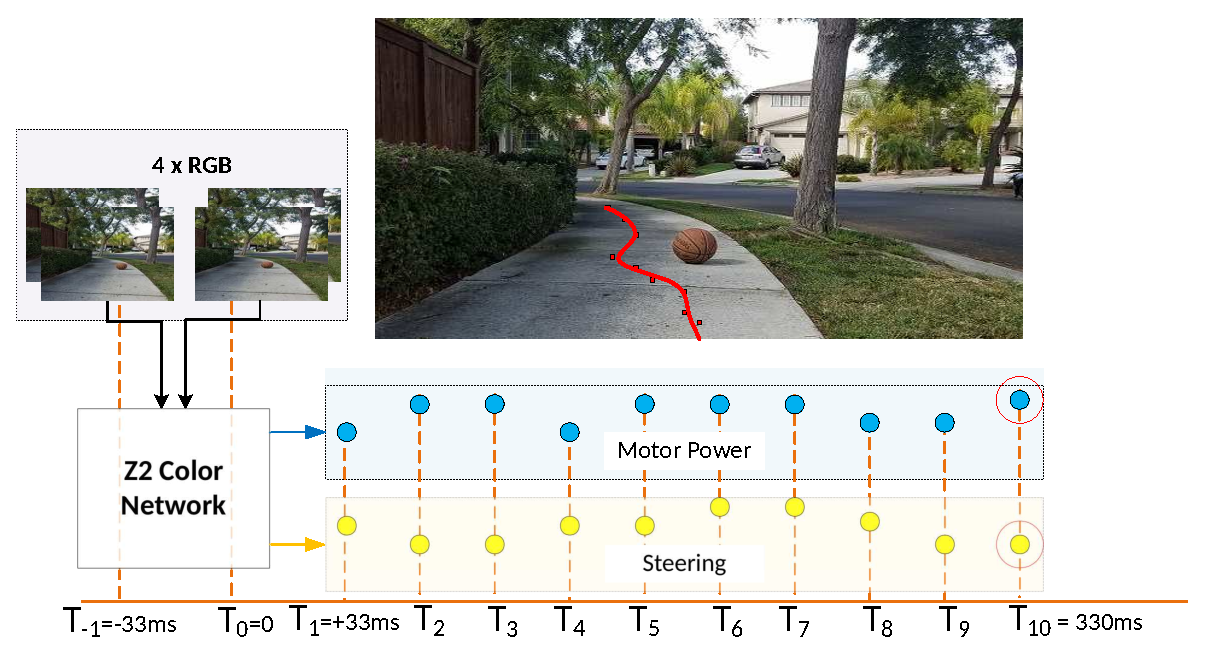
\includegraphics[width=\columnwidth]{paper/content/images/data_moment}
\caption{Data Moment}
\label{fig:moment}
\end{figure}

For perception of depth, we use left and right images from the stereo camera. To allow the network to perceive motion we use image pairs from two time steps -- one image pair gives the current position of the car, and the other is from 33 ms in the past. This way each data moment contains four RGB images.

Motor, steering, and image data are collected and stored from the car every 33 ms.
The latency between the network's prediction and actuation on the vehicle is 330 ms to mimic human reaction time. Thus the network predicts 330 ms into the future to account for this delay.

Rather than only training the network to predict a single steering and drive speed value 330 ms into the future, we instead utilize multi-task learning to improve the network's performance. To accomplish this, we train the networks to predict 10 future time steps, each 33 ms apart. In this case, only the 10th value is used for actuation and inference, while the other values serve as side-tasks to improve the cars understanding of the scene and performance on the actuated values.

The steering and motor values are floating point values ranging from zero to one. In the case of the motor values, one represents a full speed of approximately 9 meters per second. A value of zero for the motors is full speed in reverse; backward driving is used occasionally for abrupt stopping. For steering, a value of one represents the maximum steering angle towards the right, while a value of zero is the maximum steering angle towards the left.

While it is well known that the addition of such side-tasks benefits learning \cite{caruana1998multitask}, we qualitatively confirmed these improvements through on-the-road experiments. In these experiments, networks predicting only final actuation values were compared with MTL networks. It was observed that the MTL networks required far less manual correction and had greater autonomy, suggesting that the side tasks provide the network improved spatial awareness and driving capability.

\section{METHODOLOGY}
\label{sec:approach}

\begin{figure}[t]
   \centering
   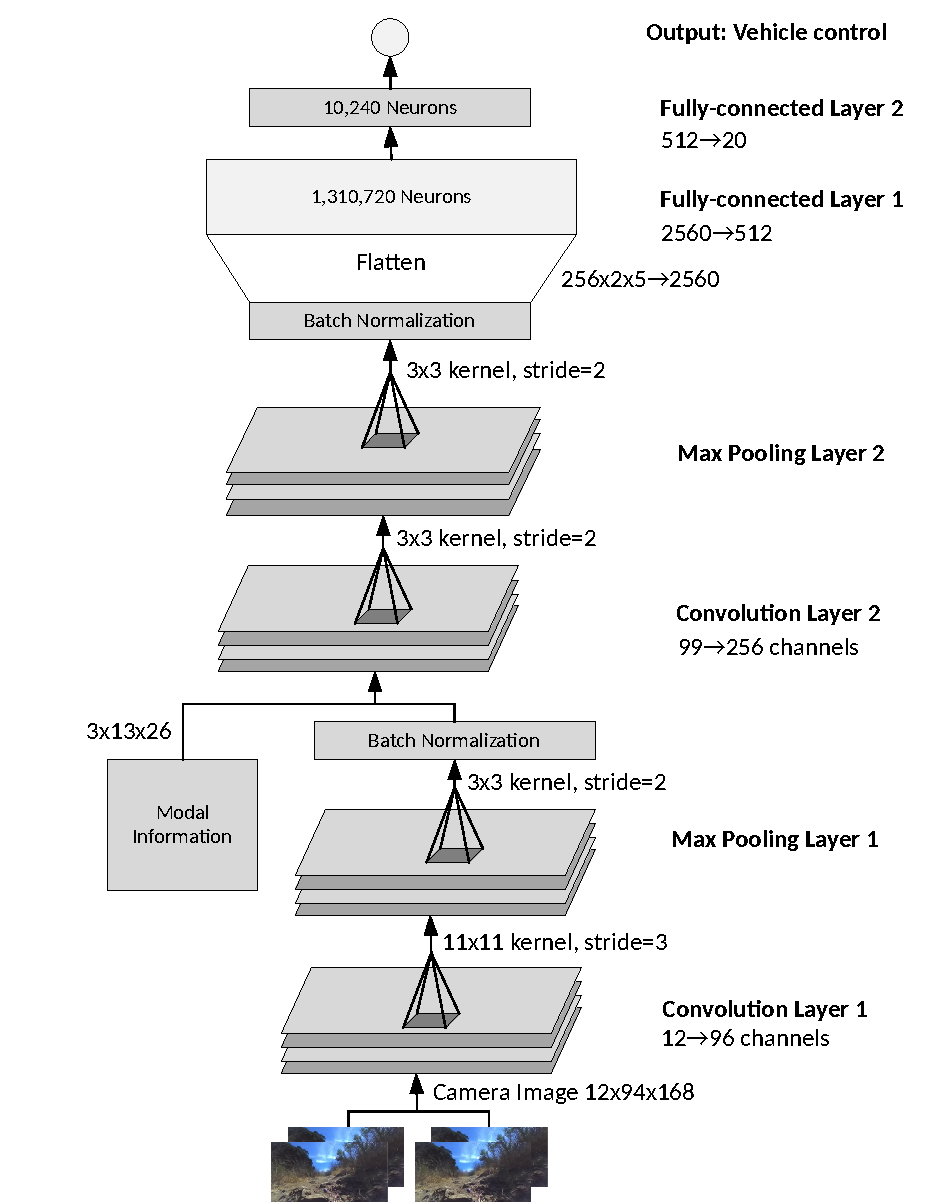
\includegraphics[width=\columnwidth,trim=0 0 20 0,clip]{paper/content/images/z2color}
   \caption{MultiNet Z2Color Network Architecture with Modal Insertion}
   \label{fig:squeeze}
\end{figure}
% Each network is trained with the Adadelta Optimizer \cite{DBLP:journals/corr/abs-1212-5701} and uses MSE Loss to compare ground truth and network output.

\subsection{Network Architecture}
For inference, we employ an NVIDIA Jetson TX1 system, and run a custom network we call Z2Color at a 20 Hz frequency. The network consists of two convolutional layers, followed by two fully connected layers shown in (\Cref{fig:squeeze}).

Max pooling and batch normalization were done after each convolutional layer. Max pooling allowed us to efficiently reduce dimensionality and batch normalization prevented internal covariate shift \cite{ioffe2015batch}. The stride and kernel sizes were found empirically through numerous cycles of training and on-road evaluation.
The convolutional layers were designed to act as feature extraction layers whereas the final fully connected layers act as a steering controller. However, the network was trained in an end-to-end manner so we did not isolate different forms of processing to specific sections of the network.

The network is compact, with no more than 1.7 million parameters, taking approximately 6.5 MB for each model, allowing for Field Programmable Gate Array (FPGA) or Application-Specific Integrated Circuit (ASIC) deployment. Iandola states ``FPGAs often have less than 10MB of on chip memory and no off-chip memory or storage. For inference, a sufficiently small model could be stored directly on the FPGA instead of being bottlenecked by memory bandwidth." \cite{DBLP:journals/corr/IandolaMAHDK16}

%In inference mode, small models have been shown to be able to be stored on FPGAs to avoid memory bandwith bottlenecks \cite{qiu2016going}. It is standard for FPGAs to contain fewer than 10 MB of block memory on the chip and no expandable memory \footnote{The popular Xilinx Vertex-7 FPGA has a maximum Total Block Ram of 8.5 MB of on chip memory with no expandable memory off-chip.} Similarly, for deployment of DNNs on ASICs, a small model is necessary to be stored directly on chip \cite{DBLP:journals/corr/IandolaMAHDK16}.

While a single MultiNet Z2Color network could fit on such a platform, multiple MTL Z2Color networks trained for just two behavioral modalities would result in a 13 MB model incapable of running directly on a 10 MB FPGA. For these reasons, as the number of modalities increases multiple distinct networks become increasingly impractical for deployment whereas a MultiNet Z2Color network allows for deployment on faster platforms with smaller network sizes.

% We wanted to choose a compact but powerful DNN, that could be run at 20 Hz or above on the NVIDIA TX1 board. The network that fit these criteria for us was SqueezeNet \cite{DBLP:journals/corr/IandolaMAHDK16}. It has been shown to match the performance of AlexNet with 500x fewer parameters in the network. It has also been shown to perform well in Autonomous Driving Tasks \cite{tusharsfuturepaper}. In order to use this network we need to make some simple modifications to the input and output of our network.

\subsection{Modal Information}

When collecting data from the cars, along with motor, steering, and image data, we also store the behavioral mode in which the car is being operated. We have trained networks with and without the insertion of the behavioral information and when added, networks more distinctly exhibit individual modal behaviors.

A network without this modal information could potentially learn multiple behavioral modes distinctly, but it would take a great amount of careful training for the filters to separate for each behavioral modality. By adding the logical modal switch in the processing stream, it becomes easier for the network to create independent filters for each behavioral mode.

The behavioral information is inserted as a three channel binary tensor, where each channel represents a different behavioral modality. In order to concatenate with the image going through the convolutional network, the behavioral information is replicated in the spatial dimensions to form a binary tensor of size 3x13x26. The behavioral mode information insertion point in the network was chosen to be after the first convolutional layer in Z2Color (\Cref{fig:squeeze}), allowing for the earlier convolutional layer to generalize basic image processing of the input data without considering behaviors of individual modalities. This replicates the processing of visual data in the macaque monkey in which the early visual cortex receives contextual information from the feedback connections of the frontal cortex from a higher visual cortex. \cite{zipser1996contextual}. Similar mode agnostic convolution or processing in initial layers of a network have been shown to be effective with multiple modalities \cite{firstlayernometa}.


\addtolength{\textheight}{-10pt}

\section{EXPERIMENTS}
\label{sec:experiments}

\subsection{Training}
To train our networks, we used the PyTorch\footnote{\url{https://github.com/pytorch/pytorch}} deep learning framework. The networks were trained using the Adadelta Optimizer \cite{DBLP:journals/corr/abs-1212-5701}.

The loss function used for training and validation was Mean Squared Error  (MSE) Loss. During the training phase, the loss was calculated across all values outputted by the network, i.e., across all ten time steps following the formula
\begin{equation}
MSE_{train} = \dfrac{1}{2n}\sum_{t=1}^{n}(s'_t -  s_t)^2 +(m'_t - m_t)^2 
\end{equation}
where $n=10$ is the number of time steps in our case, $s_t$  and $m_t$ are the steering and motor values respectively outputted by the network at a given time step, and $s'_t$ and $p'_t$ are the expert steering and motor values at a given timestep.

During validation, a similar MSE loss metric was used except the loss was calculated only for the two final motor and steering output as given by
\begin{equation}
MSE_{validation} = \dfrac{1}{2} (s'_n -  s_n)^2 +(m'_n - m_n)^2
\end{equation}
Only the final timestep was used in measuring the validation accuracy of the networks as this is the only value which is used for evaluation on the model vehicles, and thus the only value which affects the driving performance of the model car. We chose to use the MSE loss function, as small deviations from expert driving were considered normal while larger deviations are reflective of a problem in the network's control and thus have a greater effect on the calculated error. The quadratic error curve of MSE loss allows for such results and closely mimics results from the percentage autonomy metric introduced later in the paper in which small deviations have an inconsequential effect on performance.

The same set of training data were used for each of the networks, as well as the same unseen validation set. All experiments were replicated eight times with randomly initialized networks and shuffled datasets. The results here depict the mean across these trials, with error bars representing 95\% confidence intervals.

Our dataset contains approximately 1.93 million usable data moments for training and validation on the networks. 10\% of the collected data were kept for use in an unseen validation dataset for the evaluation of the networks. All data were equally distributed for each modality in both the training and validation sets. 

\subsection{Multi-Modal Comparison}
In our initial experiment a MultiNet Z2Color network trained in a multi-modal dataset of direct, follow, and furtive was compared to three MTL Z2Color networks trained on direct, follow, and furtive modes separately. Both networks were trained to output additional intermediate motor and steering values not used during inference. The three MTL networks were only fed data that corresponded to their individual behavioral modes. The MultiNet network was fed data containing all three behavioral modes. The results are summarized in \Cref{fig:lve} where the losses of the three MTL networks are averaged for direct comparison to the MultiNets.

\begin{figure}[t]
\centering
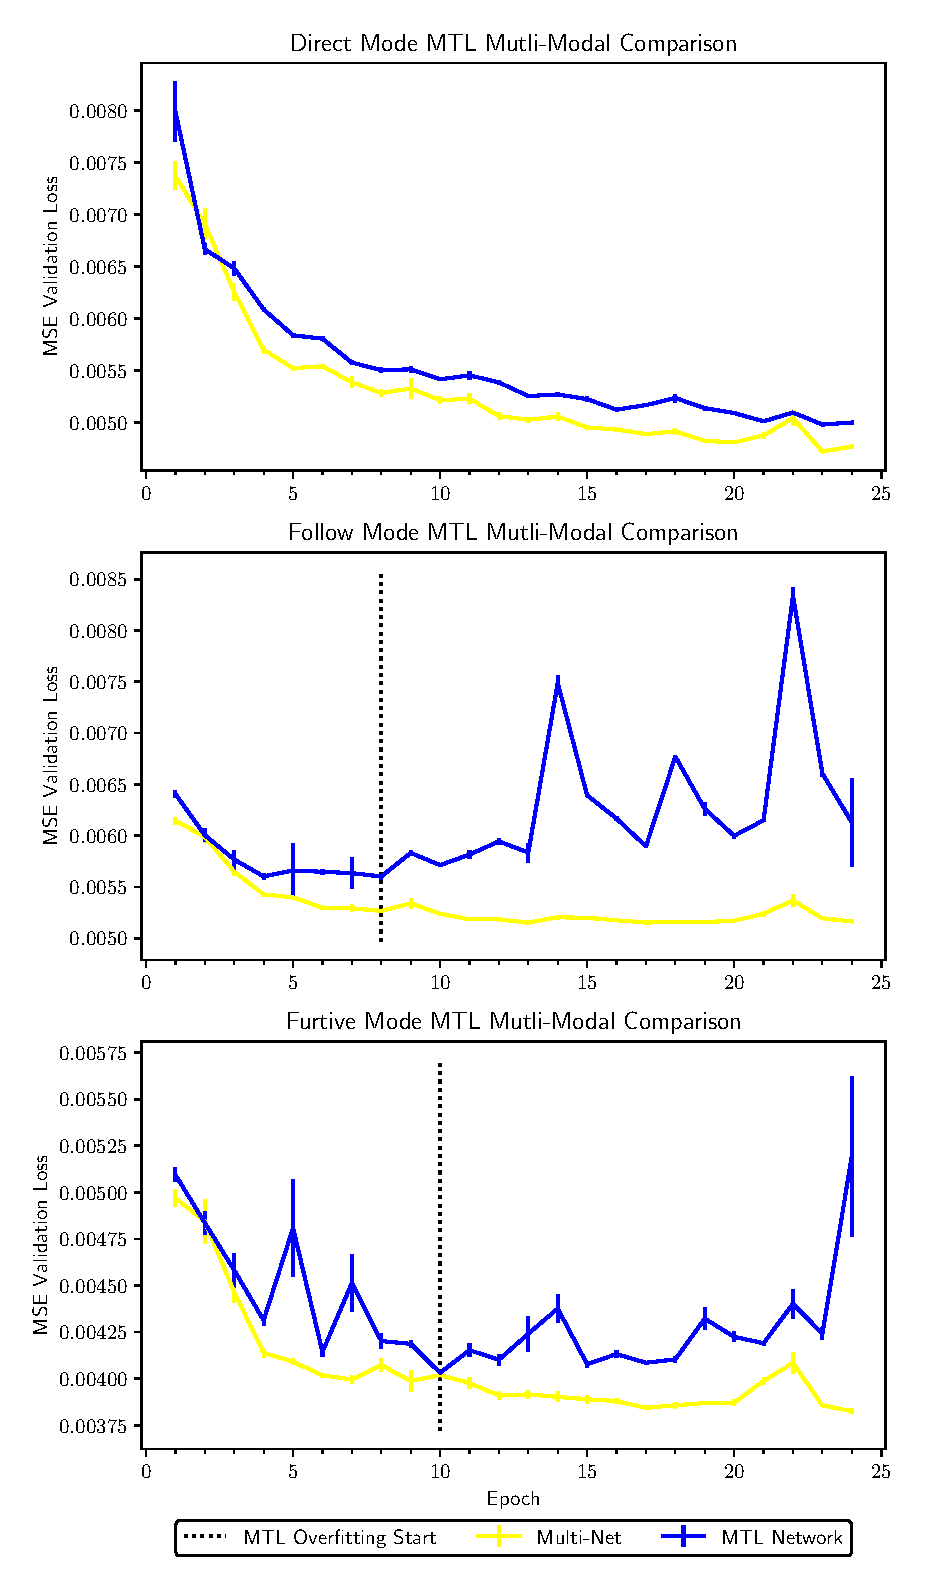
\includegraphics[width=\linewidth]{paper/content/images/individual_new}
\caption{Furtive Mode Validation of MultiNet and MTL Networks with 95\% Confidence Intervals}

\label{fig:furtivegraph}
\end{figure}

Initially, from epochs 1 to 4, the MultiNets have similar but slightly poorer performance compared to the MTL networks. This is due to the wide variety of data the MultiNets receive requiring greater generalization initially, while the MTL networks can immediately specialize to specific modes.

From epochs 4 to 10, the MultiNets begin to surpass the MTL networks while remaining close in performance. During this period the MTL networks begin to differentiate between individual driving modalities by using the provided modal information data.

From epochs 10 to 17, the MultiNets drastically outperform the MTL networks, which flatten off in their loss curve here. The MTL loss curve begins to move erratically by getting caught in various local minima. However it doesn't yet begin overfitting, which we characterize as consistently having a loss value above the absolute minimum. The MultiNets steadily improve through the use of the additional modal data. From epochs 17 to 24, the MTL networks begin to overfit dramatically, while the MultiNets continue to decline in loss despite a small bump at epochs 21 and 22. This suggests MTL networks are more susceptible to overfitting and local minima than their MultiNet counterpart.

\subsection{Performance in Individual Modes}

To further investigate the network's performance in individual behavioral modes, we decided to compare MultiNet to a single MTL network in a single mode: furtive. This mode is interesting as it involves more complex behaviors than traditional driving tasks like lane following. In these experiments (\Cref{fig:furtivegraph}), the MultiNets were trained on Direct, Follow, and Furtive modes but were only validated in Furtive mode, while the MTL net was trained and validated specifically on Furtive mode data.

Initially, from epochs 1 to 4 the MultiNets have similar performance to the furtive networks. From epochs 4 to 10, the MultiNets fall steadily in loss, while the MTL networks oscillate erratically in local minima. From epochs 10 to 24, the MTL networks overfit while the MultiNets continue learning. This demonstrates that for any given mode, a MultiNet network can outperform an MTL network trained for the specific mode.

%This mirrors the results from \Cref{fig:lve}, and confirms the MultiNets resistance to overfitting and local minima as well as their general improved performance.

\subsection{Evaluation on Model Cars}

To test the proficiency of the cars in real world driving situations, we measure the percentage autonomy metric \cite{bojarski2016end} measured as
\begin{equation}
    autonomy = (1 - \dfrac{correction\ time}{elapsed\ time}) \cdot 100
   \label{eq:autonomy}
\end{equation}

MTL and MultiNets were evaluated on a winding 200 m loop of sidewalk (\Cref{fig:evalpath}) with sufficient obstacles within a one hour interval. Follow mode was excluded as driving of the leader car could affect performance of the following car. The networks for on the road evaluation were chosen at the point of absolute minimum average validation error across the trials, i.e., we chose the epoch and trial which minimized the average validation error for both the MultiNet and MTL networks. This minimum occured at epoch 23 on a specific trial, before either network began to overfit. 

The results are summarized as follows: The MultiNet in direct, and furtive mode scored 92.68\% and 88.23\% autonomy respectively. The MTL networks scored 84.27\% and 87.55\% in direct and furtive modes. Comparatively, in direct mode the MultiNet was 8.31 \% more autonomous than the network trained only on direct mode data. In furtive mode the MultiNet was 0.68 \% more autonomous than the MTL net, matching the results from validation on furtive mode and across modes (\Cref{fig:furtivegraph,fig:lve}).

\begin{figure}[t]
\centering
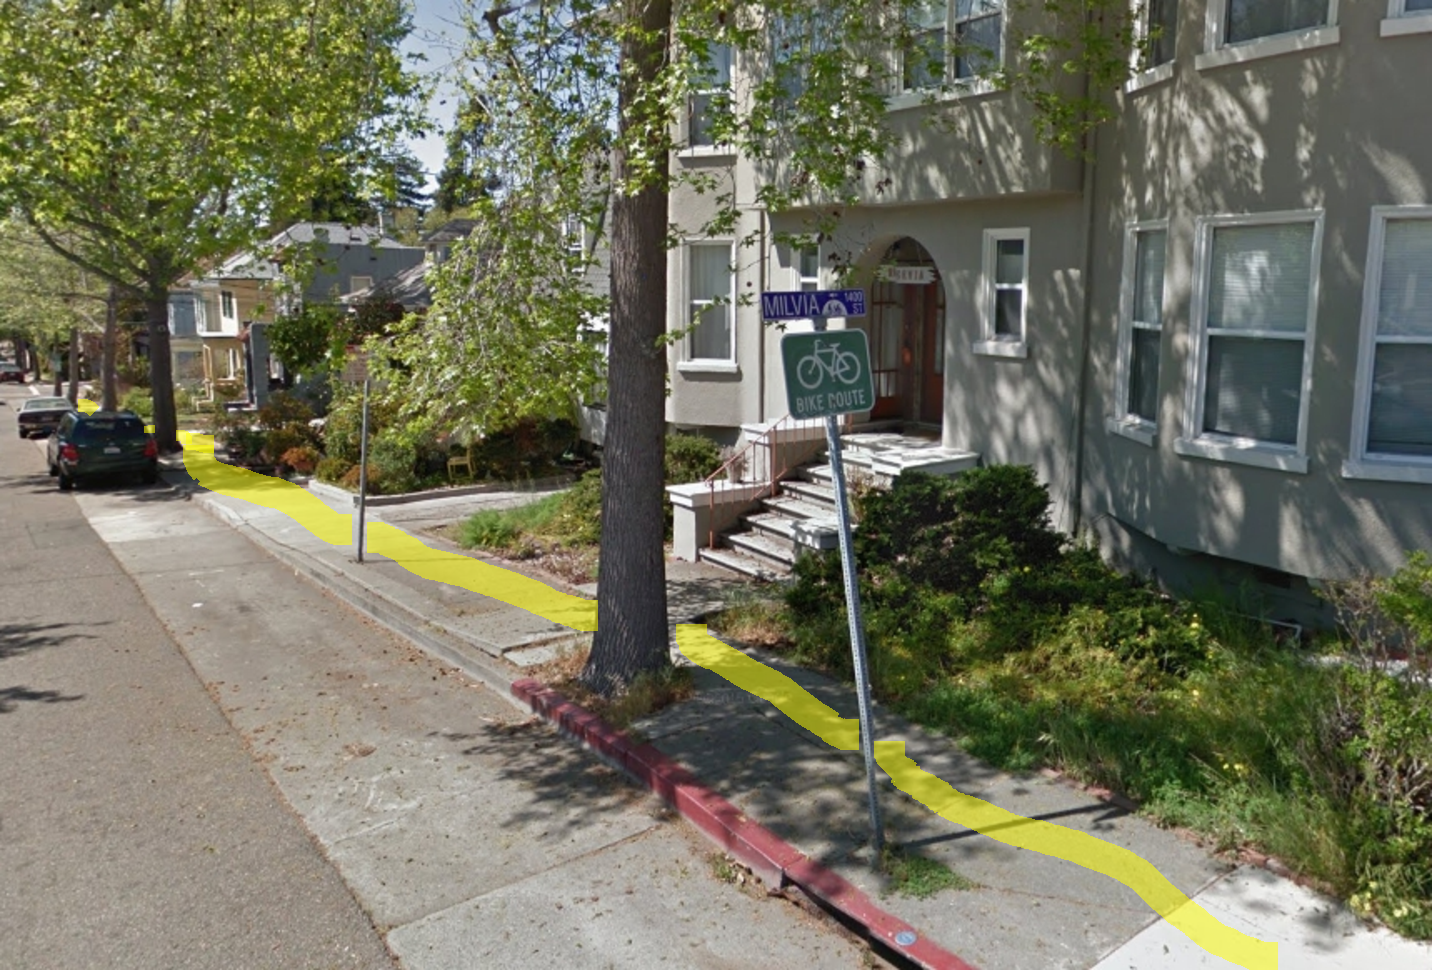
\includegraphics[width=\linewidth,,trim=0 0 0 0,clip]{paper/content/images/evaluation_path}
\caption{Segment of Evaluation Circuit}
\label{fig:evalpath}
\end{figure}

\section{CONCLUSION \& FUTURE WORKS}
\label{sec:conclusion}
This paper proposes a methodology for training DNNs to perform in several distinct behavioral modalities simultaneously, through the insertion of modal information. This MultiNet approach is shown to exceed the performance of multiple individual networks trained separately, while using fewer parameters. The MultiNet networks are shown to be more resistant to overfitting as well as capable of developing more specific behaviors characteristic of the behavioral mode of operation. These results are verified with real world evaluation of the networks in sidewalk driving situations using 1/10th scale model cars. Future work could include work on adapting the approach to full size vehicles as well as implementation of MultiNet architectures in other type of neural network models, such as recurrent networks. Additionally, in the future work could be done to make modal information available from higher-level networks trained to select behavioral modes, thereby granting the system a qualitatively higher level of autonomy.

\section*{ACKNOWLEDGMENTS}
The authors gratefully acknowledge NVIDIA for the donation of the NVIDIA TX1 Developer Kits, as well as Berkeley DeepDrive and it's sponsors for their support. We thank Sascha Hornauer and Eric Hou for their review, as well as Bhaskar Chowdhuri for assistance with figures.


{\small
\bibliographystyle{ieee}
\bibliography{egbib}
}

\end{document}
